\chapter{Preliminary study}
\lhead{\textit{Chapitre \thechapter}}
\rhead{\textit{Preliminary study}}

\section{Introduction}
Lorem ipsum dolor sit amet, consectetur adipisicing elit, sed do eiusmod
tempor incididunt ut labore et dolore magna aliqua. Ut enim ad minim veniam,
quis nostrud exercitation ullamco laboris nisi ut aliquip ex ea commodo
consequat. Duis aute irure dolor in reprehenderit in voluptate velit esse
cillum dolore eu fugiat nulla pariatur. Excepteur sint occaecat cupidatat non
proident, sunt in culpa qui officia deserunt mollit anim id est laborum.

\section{General definitions}
\subsection{Information technology}
Information technology (IT) refers to everything that businesses use computers for. 
Information technology is building communications networks for a company, 
safeguarding data and information, creating and administering databases, helping 
employees troubleshoot problems with their computers or mobile devices, or doing a 
range of other work to ensure the efficiency and security of business information 
systems. Demand for professionals in this field is high and growing, and people 
entering the field have a range of career paths to choose from.\ref{it}

\subsection{definition}
\subsection{definition}
Bla bla bla bla bla (voir Figure~\ref{fig:Allmagne}).

\section{Study of existing}
\section{Analysis of existing applications}

%+++++++++++++++++++++++++++++++++++++++++++++++++++++++++++++ 
% \begin{figure} [h!]%[htbp]
% 	\vspace*{13pt}
% 	\subfloat{\label{}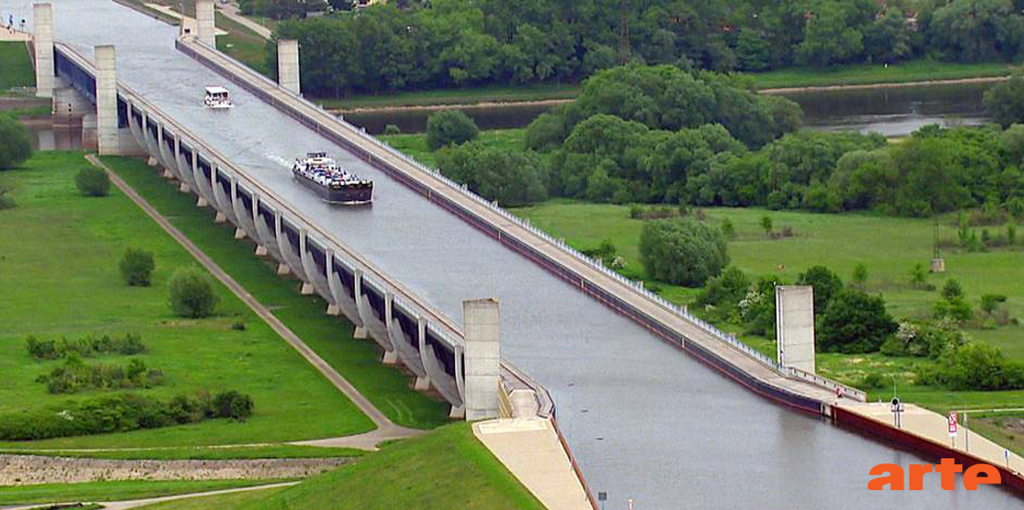
\includegraphics[scale=0.43]{img/Allmagne.png}} 
% 	\vspace*{13pt}               
% 	\caption{Titre figure 1} 
% 	\label{fig:Allmagne}
% \end{figure} 
%+++++++++++++++++++++++++++++++++++++++++++++++++++++++++++++++++++++++++++++++++++


%h, here
%t, top
%b, bottom

%Exemple d'une référence \cite{zadeh1978fuzzy}

%See Table \ref{tab:tableau1}

%\begin{table}[h!]
%\begin{center}
%	\begin{tabular}{|l|l|}
%		\hline
%		\textbf{Température en C} & \textbf{Température en F} \\
%		\hline
%		\hline
%		0 & ... \\
%		\hline
%		1 & ... \\
%		\hline
%		3 & ... \\
%		\hline
%		... & ... \\
%		\hline
%	\end{tabular}
%\end{center}
%\caption{Titre du tableau}
%\label{tab:tableau1}
%\end{table}

